% Options for packages loaded elsewhere
\PassOptionsToPackage{unicode}{hyperref}
\PassOptionsToPackage{hyphens}{url}
%
\documentclass[
  ignorenonframetext,
]{beamer}
\usepackage{pgfpages}
\setbeamertemplate{caption}[numbered]
\setbeamertemplate{caption label separator}{: }
\setbeamercolor{caption name}{fg=normal text.fg}
\beamertemplatenavigationsymbolsempty
% Prevent slide breaks in the middle of a paragraph
\widowpenalties 1 10000
\raggedbottom
\setbeamertemplate{part page}{
  \centering
  \begin{beamercolorbox}[sep=16pt,center]{part title}
    \usebeamerfont{part title}\insertpart\par
  \end{beamercolorbox}
}
\setbeamertemplate{section page}{
  \centering
  \begin{beamercolorbox}[sep=12pt,center]{part title}
    \usebeamerfont{section title}\insertsection\par
  \end{beamercolorbox}
}
\setbeamertemplate{subsection page}{
  \centering
  \begin{beamercolorbox}[sep=8pt,center]{part title}
    \usebeamerfont{subsection title}\insertsubsection\par
  \end{beamercolorbox}
}
\AtBeginPart{
  \frame{\partpage}
}
\AtBeginSection{
  \ifbibliography
  \else
    \frame{\sectionpage}
  \fi
}
\AtBeginSubsection{
  \frame{\subsectionpage}
}
\usepackage{amsmath,amssymb}
\usepackage{iftex}
\ifPDFTeX
  \usepackage[T1]{fontenc}
  \usepackage[utf8]{inputenc}
  \usepackage{textcomp} % provide euro and other symbols
\else % if luatex or xetex
  \usepackage{unicode-math} % this also loads fontspec
  \defaultfontfeatures{Scale=MatchLowercase}
  \defaultfontfeatures[\rmfamily]{Ligatures=TeX,Scale=1}
\fi
\usepackage{lmodern}
\ifPDFTeX\else
  % xetex/luatex font selection
\fi
% Use upquote if available, for straight quotes in verbatim environments
\IfFileExists{upquote.sty}{\usepackage{upquote}}{}
\IfFileExists{microtype.sty}{% use microtype if available
  \usepackage[]{microtype}
  \UseMicrotypeSet[protrusion]{basicmath} % disable protrusion for tt fonts
}{}
\makeatletter
\@ifundefined{KOMAClassName}{% if non-KOMA class
  \IfFileExists{parskip.sty}{%
    \usepackage{parskip}
  }{% else
    \setlength{\parindent}{0pt}
    \setlength{\parskip}{6pt plus 2pt minus 1pt}}
}{% if KOMA class
  \KOMAoptions{parskip=half}}
\makeatother
\usepackage{xcolor}
\newif\ifbibliography
\setlength{\emergencystretch}{3em} % prevent overfull lines
\providecommand{\tightlist}{%
  \setlength{\itemsep}{0pt}\setlength{\parskip}{0pt}}
\setcounter{secnumdepth}{-\maxdimen} % remove section numbering
%\usetheme{metropolis}


%\setbeamercolor{normal text}{bg=white}
%\addtobeamertemplate{frametitle}{}{\vspace{-0.5em}} % decrease
%\setbeamersize{text margin left=5mm,text margin right=10mm}
%\usefonttheme[onlymath]{serif}
%\usefonttheme{professionalfonts}
%%%%%%%%%%%%%%%%
% Packages
%%%%%%%%%%%%%%%%

\usepackage{geometry}
\usepackage{graphicx}
\usepackage{amssymb}
\usepackage{amsopn}
\usepackage{cancel}
\usepackage{epstopdf}
\usepackage{amsmath}  	% this permits text in eqnarray among other benefits
\usepackage{url}		% produces hyperlinks
\usepackage{hyperref}	% allows for color usage in tables
\usepackage[english]{babel}
%\usepackage[latin1]{inputenc}
\usepackage{colortbl}	% allows for color usage in tables
\usepackage{multirow}	% allows for rows that span multiple rows in tables
\usepackage{color}		% this package has a variety of color options
\usepackage{xcolor}
\usepackage{pgf}
\usepackage{calc}
\usepackage{ulem}
\usepackage{multicol}
\usepackage{booktabs}
\usepackage{textcomp}
%\usepackage[misc]{ifsym} % for the dice symbol \Cube{}
%\usepackage{txfonts}
%\usepackage{listings}
%\usepackage{tikz}
\usepackage{array}
\usepackage{wasysym}
\usepackage{fancyvrb}

%% change fontsize of R code
\ifdefined\Shaded
\let\oldShaded\Shaded
\let\endoldShaded\endShaded
\renewenvironment{Shaded}{\footnotesize\oldShaded}{\endoldShaded}
\fi
%% change fontsize of output
\let\oldverbatim\verbatim
\let\endoldverbatim\endverbatim
\renewenvironment{verbatim}{\footnotesize\oldverbatim}{\endoldverbatim}

%%%%%%%%%%%%%%%%
% Remove navigation symbols
%%%%%%%%%%%%%%%%

\setbeamertemplate{navigation symbols}{}

\setbeamertemplate{footline}[frame number]

%%%%%%%%%%%%%%%%
% User defined colors
%%%%%%%%%%%%%%%%

\xdefinecolor{oiB}{rgb}{0.22,0.52,0.72}
\definecolor{oiG}{rgb}{.298,.447,.114}
\xdefinecolor{hlblue}{rgb}{0.051,0.65,1}
\xdefinecolor{gray}{rgb}{0.5, 0.5, 0.5}
\xdefinecolor{darkGray}{rgb}{0.3, 0.3, 0.3}
\xdefinecolor{darkerGray}{rgb}{0.2, 0.2, 0.2}
\xdefinecolor{rubineRed}{rgb}{0.89,0,0.30}
\xdefinecolor{irishGreen}{rgb}{0,0.60,0}	
\definecolor{lightGreen}{rgb}{0.387,0.581,0.148}

%%%%%%%%%%%%%%%%
% Template colors
%%%%%%%%%%%%%%%%

%\setbeamercolor*{palette primary}{fg=white,bg= oiB!80!black!90}
%\setbeamercolor*{palette secondary}{fg=black,bg= oiB!80!black}
%\setbeamercolor*{palette tertiary}{fg=white,bg= oiB!80!black!80}
%\setbeamercolor*{palette quaternary}{fg=white,bg= oiB}
%\setbeamercolor{structure}{fg= oiB}
%\setbeamercolor{frametitle}{bg= oiB!90}
%\setbeamertemplate{blocks}[shadow=false]
%\setbeamersize{text margin left=2em,text margin right=2em}

%\setbeamercolor{code body}{bg=gray!20!white!80,fg=black}


%%%%%%%%%%%%%%%%
% Get rid of fancy enumerated list bullets
%%%%%%%%%%%%%%%%

%\setbeamertemplate{enumerate items}[default]

%%%%%%%%%%%%%%%%
% Custom commands
%%%%%%%%%%%%%%%%

\newcommand{\Sum}{\sum\nolimits}
\newcommand{\Hide}[2]{\underline{~~~\onslide<#1>{\alert{#2}}~~~}}
\newcommand{\hide}[2]{\underline{~~\onslide<#1>{\alert{#2}}~~}}
\newcommand{\hid}[2]{\onslide<#1>{\alert{#2}}}
\newcommand{\code}[1]{\textcolor{blue}{\texttt{#1}}}

% red
\newcommand{\red}[1]{\textit{\textcolor{rubineRed}{#1}}}

% pink
\newcommand{\pink}[1]{\textit{\textcolor{rubineRed!90!white!50}{#1}}}

% green
\newcommand{\green}[1]{\textit{\textcolor{irishGreen}{#1}}}

% orange
\newcommand{\orange}[1]{\textit{\textcolor{orange}{#1}}}

% links: webURL, webLin, appLink
\newcommand{\webURL}[1]{\urlstyle{same}{ \textit{\textcolor{darkGray}{\url{#1}}}}}
\newcommand{\webLink}[2]{\href{#1}{\textcolor{darkGray}{{#2}}}}
\newcommand{\appLink}[2]{\href{#1}{\textcolor{white}{{#2}}}}

% mail
\newcommand{\mail}[1]{\href{mailto:#1}{\textit{\textcolor{darkGray}{#1}}}}

% highlighting: hl, hlGr, mathhl
\newcommand{\hl}[1]{\textit{\textcolor{hlblue}{#1}}}
\newcommand{\hlGr}[1]{\textit{\textcolor{lightGreen}{#1}}}
\newcommand{\mathhl}[1]{\textcolor{hlblue}{\ensuremath{#1}}}

% two col: two columns
\newenvironment{twocol}[4]{
\begin{columns}[c]
\column{#1\textwidth}
#3
\column{#2\textwidth}
#4
\end{columns}
}





%%%%%%%%%%%%%%%%
% Change margin
%%%%%%%%%%%%%%%%

\newenvironment{changemargin}[2]{%
\begin{list}{}{%
\setlength{\topsep}{0pt}%
\setlength{\leftmargin}{#1}%
\setlength{\rightmargin}{#2}%
\setlength{\listparindent}{\parindent}%
\setlength{\itemindent}{\parindent}%
\setlength{\parsep}{\parskip}%
}%
\item}{\end{list}}

%%%%%%%%%%%%%%%%
% Footnote
%%%%%%%%%%%%%%%%

\long\def\symbolfootnote[#1]#2{\begingroup%
\def\thefootnote{\fnsymbol{footnote}}\footnote[#1]{#2}\endgroup}

%%%%%%%%%%%%%%%%
% Graphics
%%%%%%%%%%%%%%%%

\DeclareGraphicsRule{.tif}{png}{.png}{`convert #1 `dirname #1`/`basename #1 .tif`.png}



\setbeamercolor{normal text}{bg=white}

\DeclareMathOperator{\var}{var}
\newcommand{\boxmodel}[1]{\begin{array}{|c|}#1\\[2pt]\hline\end{array}}
\newcommand{\BXX}[2]{\begin{array}{|@{\,}c@{\,}|@{\,}c@{\,}|}\hline#1&#2\\[-1pt]\hline\end{array}}
\newcommand{\p}{\mathrm{P}}
\newcommand{\SE}{\mathrm{SE}}
\newcommand{\xbar}{\overline{x}}
\newcommand{\Xbar}{\overline{X}}
\newcommand{\ybar}{\overline{y}}
\newcommand{\Ybar}{\overline{Y}}
\newcommand{\zbar}{\overline{z}}
\newcommand{\Zbar}{\overline{Z}}
\newcommand{\wbar}{\overline{w}}
\newcommand{\Wbar}{\overline{W}}
\newcommand{\vbar}{\overline{v}}
\newcommand{\Vbar}{\overline{V}}
\newcommand{\dbar}{\overline{d}}
\newcommand{\Dbar}{\overline{D}}
\newcommand{\ebar}{\overline{e}}
\newcommand{\ehat}{\widehat{\epsilon}}
\newcommand{\yhat}{\widehat{y}}
\newcommand{\Yhat}{\widehat{Y}}
\newcommand{\bhat}{\widehat{\beta}}
\newcommand{\dl}[1]{\widehat{\delta}_{#1}}
\newcommand{\g}[1]{\widehat{\gamma}_{#1}}
\newcommand{\al}[1]{\widehat{\alpha}_{#1}}
\newcommand{\Bj}{{\beta_j}}
\newcommand{\Bp}{{\beta_p}}
\newcommand{\Bq}{{\beta_q}}
\renewcommand{\b}[1]{\widehat{\beta}_{#1}}
\newcommand{\B}[1]{{\beta}_{#1}}
\newcommand{\BETA}{{\boldsymbol\beta}}
\newcommand{\bp}{\widehat{\beta}_p}
\newcommand{\bq}{\widehat{\beta}_q}
\newcommand{\bj}{\widehat{\beta}_j}
\newcommand{\df}{\mathrm{df}}
\DeclareMathOperator{\VIF}{VIF}
\DeclareMathOperator{\SSE}{SSE}
\DeclareMathOperator{\SST}{SST}
\DeclareMathOperator{\SSR}{SSR}
\DeclareMathOperator{\MSE}{MSE}
\DeclareMathOperator{\MST}{MST}
\DeclareMathOperator{\MSR}{MSR}
\DeclareMathOperator{\RM}{RM}
\DeclareMathOperator{\FM}{FM}
\DeclareMathOperator{\E}{E}
\DeclareMathOperator{\SD}{SD}
\DeclareMathOperator{\se}{se}
\DeclareMathOperator{\cov}{Cov}
\DeclareMathOperator{\corr}{Corr}
\DeclareMathOperator{\cor}{Cor}
\DeclareMathOperator{\Var}{Var}
\DeclareMathOperator{\logit}{logit}
\newcommand{\hsigma}{\widehat{\sigma}}
\newcommand{\betahat}{\widehat{\beta}}
\newcommand{\slide}{<br><br><br><br><br>}
\newcommand{\bbeta}{\boldsymbol{\beta}}
\newcommand{\bX}{\mathbf{X}}
\newcommand{\bY}{\mathbf{Y}}
\newcommand{\bH}{\mathbf{H}}
\newcommand{\bI}{\mathbf{I}}
\newcommand{\be}{\mathbf{e}}
\newcommand{\pval}{\mathit{P}\mathrm{-val}}



\newcommand{\vmu}{\mbox{\boldmath{$\mu$}}}
\newcommand{\vR}{\mbox{\boldmath{$R$}}}
\newcommand{\vpsi}{\mbox{\boldmath{$\psi$}}}
\newcommand{\vZ}{\mbox{\boldmath{$Z$}}}
\newcommand{\vX}{\mbox{\boldmath{$X$}}}
\newcommand{\vY}{\mbox{\boldmath{$Y$}}}
\newcommand{\vW}{\mbox{\boldmath{$W$}}}
\newcommand{\vz}{\mbox{\boldmath{$z$}}}
\newcommand{\vr}{\mbox{\boldmath{$r$}}}
\newcommand{\vx}{\mbox{\boldmath{$x$}}}
\newcommand{\vk}{\mbox{\boldmath{$k$}}}
\newcommand{\vp}{\mbox{\boldmath{$p$}}}
\newcommand{\vv}{\mbox{\boldmath{$v$}}}
\newcommand{\vg}{\mbox{\boldmath{$g$}}}
\newcommand{\vbeta}{\mbox{\boldmath{$\beta$}}}
\newcommand{\vone}{\mbox{\boldmath{$1$}}}
\newcommand{\vep}{\mbox{\boldmath{$\epsilon$}}}
\newcommand{\veta}{\mbox{\boldmath{$\eta$}}}
\newcommand{\vl}{\mbox{\boldmath{$l$}}}
\newcommand{\ve}{\mbox{\boldmath{$e$}}}
\newcommand{\va}{\mbox{\boldmath{$a$}}}
\newcommand{\vb}{\mbox{\boldmath{$b$}}}
\newcommand{\vPsi}{\mbox{\boldmath{$\Psi$}}}
\DeclareMathOperator*{\V}{\mathbb{V}}


% geometry: topsep=0pt 
\ifLuaTeX
  \usepackage{selnolig}  % disable illegal ligatures
\fi
\IfFileExists{bookmark.sty}{\usepackage{bookmark}}{\usepackage{hyperref}}
\IfFileExists{xurl.sty}{\usepackage{xurl}}{} % add URL line breaks if available
\urlstyle{same}
\hypersetup{
  pdftitle={STAT 20000 Chapter 5The Normal Approximation for Data},
  hidelinks,
  pdfcreator={LaTeX via pandoc}}

\title{STAT 20000 Chapter 5\newline The Normal Approximation for Data}
\author{}
\date{\vspace{-2.5em}}

\begin{document}
\frame{\titlepage}

\begin{frame}{}
\protect\hypertarget{section}{}
When a histogram is bell-shaped, the \textit{approximate} values of
percentile can be found in a \textit{simple} way\newline \quad ---
approximating the histogram by a \textbf{normal curve}.

\begin{center}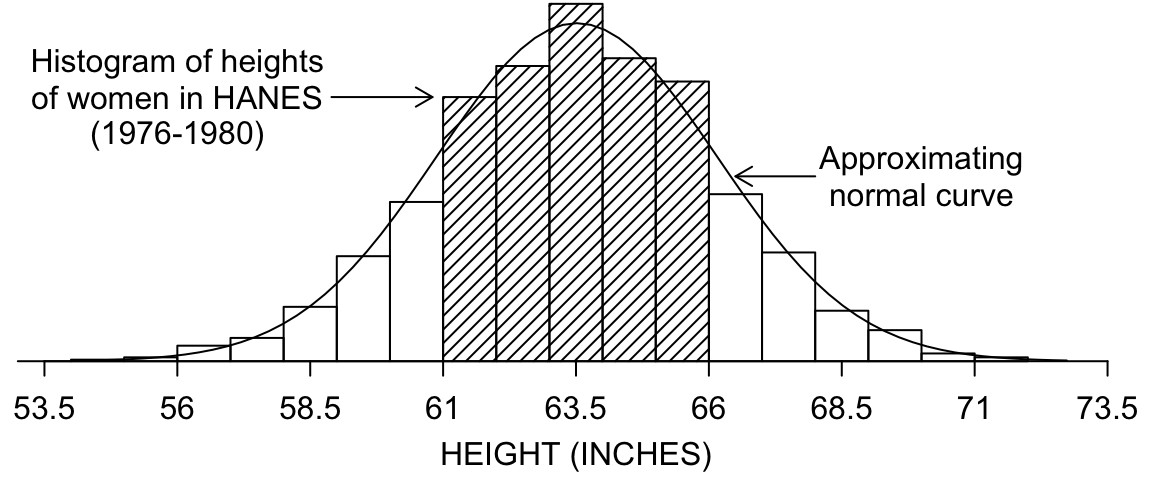
\includegraphics[width=1\linewidth]{ch05_24spr_ex_files/figure-beamer/HANESh-1} \end{center}
\end{frame}

\begin{frame}{Why Are Normal Curves of Interest?}
\protect\hypertarget{why-are-normal-curves-of-interest}{}
\begin{enumerate}
\item
  Many variables (e.g., height, blood pressure, \dots, but not years of
  education, \dots) have histograms which follow (match up well with) a
  normal curve.\bigskip
\item
  For such variables, areas under the histogram --- that is, population
  percentages --- can be approximated by the corresponding areas under
  the normal curve:
\end{enumerate}

\begin{center}
\includegraphics[width=1\linewidth]{ch05_24spr_ex_files/figure-beamer/unnamed-chunk-5-1} \end{center}
\end{frame}

\begin{frame}{Why Are Normal Curves of Interest? (Cont'd)}
\protect\hypertarget{why-are-normal-curves-of-interest-contd}{}
\begin{enumerate}
\setcounter{enumi}{2}
\tightlist
\item
  Areas under the normal curve can be computed easily knowing only the
  \red{average} and the \red{SD}.
\item
  Normal curves are well known and well understood.

  \begin{itemize}
  \tightlist
  \item
    A convenient means of communication.
  \end{itemize}
\item
  The probability histogram of the averages of large samples tends to
  follow the normal curve (Central Limit Theorem, Chapter 18).

  \begin{itemize}
  \tightlist
  \item
    The cornerstone of statistical inference!
  \end{itemize}
\end{enumerate}
\end{frame}

\begin{frame}{The Standard Normal Curve}
\protect\hypertarget{the-standard-normal-curve}{}
\begin{center}
\includegraphics[width=0.85\linewidth]{ch05_24spr_ex_files/figure-beamer/unnamed-chunk-6-1} \end{center}

\begin{itemize}
\tightlist
\item
  The equation of the curve:
  \(\displaystyle{y = \frac{100\%}{\sqrt{2\pi}} \, e^{-x^2/2}}\)
\item
  Two very important properties are:

  \begin{enumerate}
  \tightlist
  \item
    The total area under the curve is \textbf{100\%},\newline \quad ---
    just like a histogram.
  \item
    The curve is \textbf{symmetric} about 0.
  \end{enumerate}
\end{itemize}
\end{frame}

\begin{frame}{A Brief Table of Areas under the Standard Normal Curve}
\protect\hypertarget{a-brief-table-of-areas-under-the-standard-normal-curve}{}
\begin{center}
\includegraphics[width=1\linewidth]{ch05_24spr_ex_files/figure-beamer/unnamed-chunk-7-1} \end{center}
\end{frame}

\begin{frame}{}
\protect\hypertarget{section-1}{}
\begin{columns}[T]
\begin{column}{.4\textwidth}
\textbf{Normal Table}

FPP, page A-155

\begin{center}
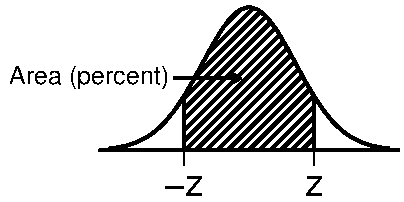
\includegraphics[width=\textwidth]{./C05/NormTab.pdf}
\end{center}

We will \red{NOT} use this FPP normal table.\bigskip

We will use the more commonly used normal table on the next page 
instead!

\end{column}
\begin{column}{.6\textwidth}
\tiny
\begin{tabular}{cccccccc}
{\footnotesize $z$} & {\footnotesize Area} &&  {\footnotesize $z$} & {\footnotesize Area} && {\footnotesize $z$} & {\footnotesize Area}  \\
\cmidrule(rl){1-2}\cmidrule(rl){4-5}\cmidrule(rl){7-8}
0.00 & ~0.~~ &&  1.50 & 86.64 &&  3.00 & 99.730~ \\
0.05 & ~3.99 &&  1.55 & 87.89 &&  3.05 & 99.771~ \\
0.10 & ~7.97 &&  1.60 & 89.04 &&  3.10 & 99.806~ \\
0.15 & 11.92 &&  1.65 & 90.11 &&  3.15 & 99.837~ \\
0.20 & 15.85 &&  1.70 & 91.09 &&  3.20 & 99.863~ \\[+3pt]

0.25 & 19.74 &&  1.75 & 91.99 &&  3.25 & 99.885~ \\
0.30 & 23.58 &&  1.80 & 92.81 &&  3.30 & 99.903~ \\
0.35 & 27.37 &&  1.85 & 93.57 &&  3.35 & 99.919~ \\
0.40 & 31.08 &&  1.90 & 94.26 &&  3.40 & 99.933~ \\
0.45 & 34.73 &&  1.95 & 94.88 &&  3.45 & 99.944~ \\[+3pt]

0.50 & 38.29 &&  2.00 & 95.45 &&  3.50 & 99.953~ \\
0.55 & 41.77 &&  2.05 & 95.96 &&  3.55 & 99.961~ \\
0.60 & 45.15 &&  2.10 & 96.43 &&  3.60 & 99.968~ \\
0.65 & 48.43 &&  2.15 & 96.84 &&  3.65 & 99.974~ \\
0.70 & 51.61 &&  2.20 & 97.22 &&  3.70 & 99.978~ \\[+3pt]

0.75 & 54.67 &&  2.25 & 97.56 &&  3.75 & 99.982~ \\
0.80 & 57.63 &&  2.30 & 97.86 &&  3.80 & 99.986~ \\
0.85 & 60.47 &&  2.35 & 98.12 &&  3.85 & 99.988~ \\
0.90 & 63.19 &&  2.40 & 98.36 &&  3.90 & 99.990~ \\
0.95 & 65.79 &&  2.45 & 98.57 &&  3.95 & 99.992~ \\[+3pt]

1.00 & 68.27 &&  2.50 & 98.76 &&  4.00 & 99.9937 \\
1.05 & 70.63 &&  2.55 & 98.92 &&  4.05 & 99.9949 \\
1.10 & 72.87 &&  2.60 & 99.07 &&  4.10 & 99.9959 \\
1.15 & 74.99 &&  2.65 & 99.20 &&  4.15 & 99.9967 \\
1.20 & 76.99 &&  2.70 & 99.31 &&  4.20 & 99.9973 \\[+3pt]

1.25 & 78.87 &&  2.75 & 99.40 &&  4.25 & 99.9979 \\
1.30 & 80.64 &&  2.80 & 99.49 &&  4.30 & 99.9983 \\
1.35 & 82.30 &&  2.85 & 99.56 &&  4.35 & 99.9986 \\
1.40 & 83.85 &&  2.90 & 99.63 &&  4.40 & 99.9989 \\
1.45 & 85.29 &&  2.95 & 99.68 &&  4.45 & 99.9991 \\
\end{tabular}
\normalsize
\end{column}
\end{columns}
\end{frame}

\begin{frame}{}
\protect\hypertarget{section-2}{}
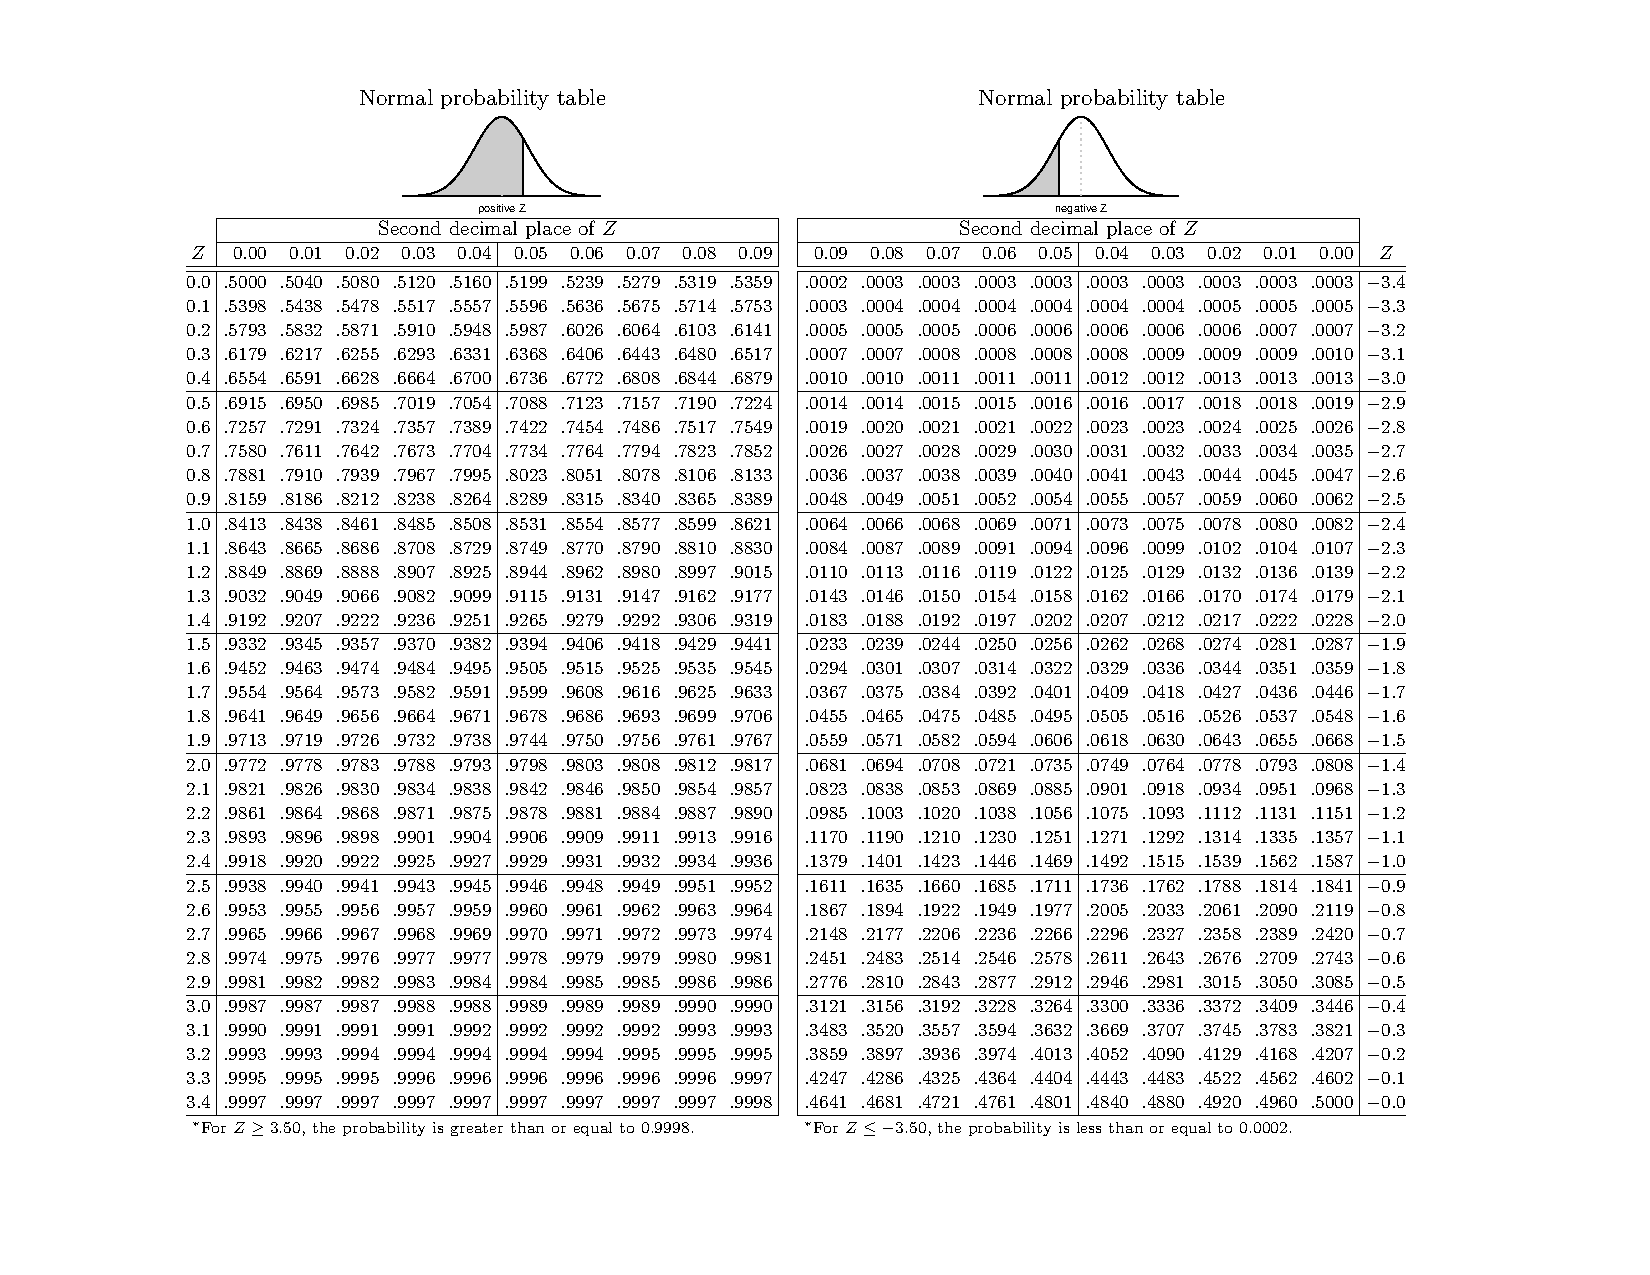
\includegraphics[width=\textwidth]{./C05/OIS3_NormTab.pdf}
\end{frame}

\begin{frame}{}
\protect\hypertarget{section-3}{}
\begin{minipage}{0.72\textwidth}
The \hl{normal probability table} on the previous slide gives
the \red{\textbf{area} under the standard normal curve to the \textbf{left} of $z$}.
\end{minipage}
\vspace{-0.7in}

\begin{flushright}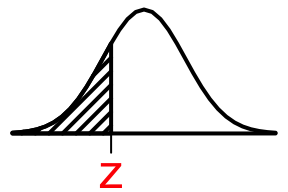
\includegraphics[width=0.25\linewidth]{ch05_24spr_ex_files/figure-beamer/NormTab-1} \end{flushright}

\centerline{
\tabcolsep=4pt\scriptsize
\only<1|handout:0>{
\begin{tabular}{@{}c|cccccccccc@{}}\hline
\textcolor{red}{\normalsize z}
      & {\footnotesize .00}   & {\footnotesize .01}   & {\footnotesize .02}   & {\footnotesize .03} & {\footnotesize .04}   & {\footnotesize .05} & {\footnotesize .06}   & {\footnotesize .07}   & {\footnotesize .08}   & {\footnotesize .09} \\\hline
$-3.4$& .0003 & .0003 & .0003 & .0003 & .0003 & .0003 & .0003 & .0003 & .0003 & .0002\\
%$-3.3$& .0005 & .0005 & .0005 & .0004 & .0004 & .0004 & .0004 & .0004 & .0004 & .0003\\
%$-3.2$& .0007 & .0007 & .0006 & .0006 & .0006 & .0006 & .0006 & .0005 & .0005 & .0005\\
%$-3.1$& .0010 & .0009 & .0009 & .0009 & .0008 & .0008 & .0008 & .0008 & .0007 & .0007\\
%$-3.0$& .0013 & .0013 & .0013 & .0012 & .0012 & .0011 & .0011 & .0011 & .0010 & .0010\\\hline
%$-2.9$& .0019 & .0018 & .0018 & .0017 & .0016 & .0016 & .0015 & .0015 & .0014 & .0014\\
%$-2.8$& .0026 & .0025 & .0024 & .0023 & .0023 & .0022 & .0021 & .0021 & .0020 & .0019\\
%$-2.7$& .0035 & .0034 & .0033 & .0032 & .0031 & .0030 & .0029 & .0028 & .0027 & .0026\\
%$-2.6$& .0047 & .0045 & .0044 & .0043 & .0041 & .0040 & .0039 & .0038 & .0037 & .0036\\
%$-2.5$& .0062 & .0060 & .0059 & .0057 & .0055 & .0054 & .0052 & .0051 & .0049 & .0048\\%\hline
%$-2.4$& .0082 & .0080 & .0078 & .0075 & .0073 & .0071 & .0069 & .0068 & .0066 & .0064\\
%$-2.3$& .0107 & .0104 & .0102 & .0099 & .0096 & .0094 & .0091 & .0089 & .0087 & .0084\\
%$-2.2$& .0139 & .0136 & .0132 & .0129 & .0125 & .0122 & .0119 & .0116 & .0113 & .0110\\
%$-2.1$& .0179 & .0174 & .0170 & .0166 & .0162 & .0158 & .0154 & .0150 & .0146 & .0143\\
%$-2.0$& .0228 & .0222 & .0217 & .0212 & .0207 & .0202 & .0197 & .0192 & .0188 & .0183\\\hline
%$-1.9$& .0287 & .0281 & .0274 & .0268 & .0262 & .0256 & .0250 & .0244 & .0239 & .0233\\
%$-1.8$& .0359 & .0351 & .0344 & .0336 & .0329 & .0322 & .0314 & .0307 & .0301 & .0294\\
%$-1.7$& .0446 & .0436 & .0427 & .0418 & .0409 & .0401 & .0392 & .0384 & .0375 & .0367\\
%$-1.6$& .0548 & .0537 & .0526 & .0516 & .0505 & .0495 & .0485 & .0475 & .0465 & .0455\\
%$-1.5$& .0668 & .0655 & .0643 & .0630 & .0618 & .0606 & .0594 & .0582 & .0571 & .0559\\\hline
%$-1.4$& .0808 & .0793 & .0778 & .0764 & .0749 & .0735 & .0721 & .0708 & .0694 & .0681\\
%$-1.3$& .0968 & .0951 & .0934 & .0918 & .0901 & .0885 & .0869 & .0853 & .0838 & .0823\\
%$-1.2$& .1151 & .1131 & .1112 & .1093 & .1075 & .1056 & .1038 & .1020 & .1003 & .0985\\
%$-1.1$& .1357 & .1335 & .1314 & .1292 & .1271 & .1251 & .1230 & .1210 & .1190 & .1170\\
$\vdots$&$\vdots$&$\vdots$&$\vdots$&$\vdots$&$\vdots$&$\vdots$&$\vdots$&$\vdots$&$\vdots$&$\vdots$\\
$-1.0$& .1587 & .1562 & .1539 & .1515 & .1492 & .1469 & .1446 & .1423 & .1401 & .1379\\%\hline
$-0.9$& .1841 & .1814 & .1788 & .1762 & .1736 & .1711 & .1685 & .1660 & .1635 & .1611\\
$-0.8$& .2119 & .2090 & .2061 & .2033 & .2005 & .1977 & .1949 & .1922 & .1894 & .1867\\
$-0.7$& .2420 & .2389 & .2358 & .2327 & .2296 & .2266 & .2236 & .2206 & .2177 & .2148\\
$-0.6$& .2743 & .2709 & .2676 & .2643 & .2611 & .2578 & .2546 & .2514 & .2483 & .2451\\
$\vdots$&$\vdots$&$\vdots$&$\vdots$&$\vdots$&$\vdots$&$\vdots$&$\vdots$&$\vdots$&$\vdots$&$\vdots$\\
$-0.0$& .5000 & .4960 & .4920 & .4880 & .4840 & .4801 & .4761 & .4721 & .4681 & .4641\\\hline
\end{tabular}
}
\only<2->{
\begin{tabular}{@{}c|ccc>{\columncolor[gray]{0.7}[1pt]}ccccccc@{}}\hline
\textcolor{red}{\normalsize z}
      & {\footnotesize .00}   & {\footnotesize .01}   & {\footnotesize .02}   & {\footnotesize .03} & {\footnotesize .04}   & {\footnotesize .05} & {\footnotesize .06}   & {\footnotesize .07}   & {\footnotesize .08}   & {\footnotesize .09} \\\hline
$-3.4$& .0003 & .0003 & .0003 & .0003 & .0003 & .0003 & .0003 & .0003 & .0003 & .0002\\
$\vdots$&$\vdots$&$\vdots$&$\vdots$&$\vdots$&$\vdots$&$\vdots$&$\vdots$&$\vdots$&$\vdots$&$\vdots$\\
$-1.0$& .1587 & .1562 & .1539 & .1515 & .1492 & .1469 & .1446 & .1423 & .1401 & .1379\\%\hline
$-0.9$& .1841 & .1814 & .1788 & .1762 & .1736 & .1711 & .1685 & .1660 & .1635 & .1611\\
\rowcolor[gray]{0.7}$-0.8$& .2119 & .2090 & .2061 & \alert{.2033} & .2005 & .1977 & .1949 & .1922 & .1894 & .1867\\
$-0.7$& .2420 & .2389 & .2358 & .2327 & .2296 & .2266 & .2236 & .2206 & .2177 & .2148\\
$-0.6$& .2743 & .2709 & .2676 & .2643 & .2611 & .2578 & .2546 & .2514 & .2483 & .2451\\ $\vdots$&$\vdots$&$\vdots$&$\vdots$&$\vdots$&$\vdots$&$\vdots$&$\vdots$&$\vdots$&$\vdots$&$\vdots$\\
$-0.0$& .5000 & .4960 & .4920 & .4880 & .4840 & .4801 & .4761 & .4721 & .4681 & .4641\\\hline
\end{tabular}
}
}\normalsize

E.g., for \(z=-0.83\), look at the row \(-0.8\) and the column 0.03.

\begin{center}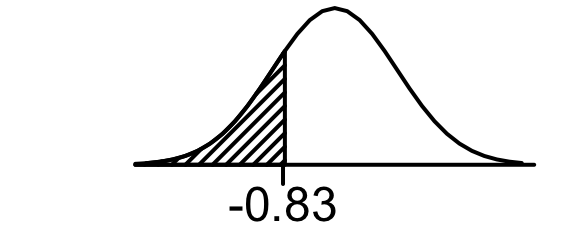
\includegraphics[width=0.35\linewidth]{ch05_24spr_ex_files/figure-beamer/normm083-1} \end{center}
\vspace{-0.65in}
\begin{center}
Shaded Area $=$\hspace{.25\textwidth}
= \hide{2-}{0.2033}
\end{center}
\end{frame}

\begin{frame}{In-Class Exercise 1a}
\protect\hypertarget{in-class-exercise-1a}{}
Find the area under the standard normal curve to the left of \(-0.97\).
\pause

\begin{center}
\includegraphics[width=0.45\linewidth]{ch05_24spr_ex_files/figure-beamer/unnamed-chunk-8-1} \end{center}
\scriptsize
\tabcolsep=3pt

\begin{tabular}[t]{l|r|r|>{}r|r|r|r|r|r|r|r}
\hline
  & 0.09 & 0.08 & 0.07 & 0.06 & 0.05 & 0.04 & 0.03 & 0.02 & 0.01 & 0.00\\
\hline
-1 & 0.1379 & 0.1401 & \cellcolor{lightgray}{0.1423} & 0.1446 & 0.1469 & 0.1492 & 0.1515 & 0.1539 & 0.1562 & 0.1587\\
\hline
\cellcolor{lightgray}{-0.9} & \cellcolor{lightgray}{0.1611} & \cellcolor{lightgray}{0.1635} & \cellcolor{lightgray}{0.1660} & \cellcolor{lightgray}{0.1685} & \cellcolor{lightgray}{0.1711} & \cellcolor{lightgray}{0.1736} & \cellcolor{lightgray}{0.1762} & \cellcolor{lightgray}{0.1788} & \cellcolor{lightgray}{0.1814} & \cellcolor{lightgray}{0.1841}\\
\hline
-0.8 & 0.1867 & 0.1894 & \cellcolor{lightgray}{0.1922} & 0.1949 & 0.1977 & 0.2005 & 0.2033 & 0.2061 & 0.2090 & 0.2119\\
\hline
\end{tabular}

\normalsize

Ans: 0.1660
\end{frame}

\begin{frame}{}
\protect\hypertarget{section-4}{}
\vspace{4pt}
\begin{minipage}{0.75\textwidth}
\textbf{Question}:
Find the \textbf{area} under the standard\newline
normal curve to the \textbf{left} of 1.573.
\end{minipage}
\vspace{-0.5in}

\begin{flushright}
\includegraphics[width=0.22\linewidth]{ch05_24spr_ex_files/figure-beamer/unnamed-chunk-10-1} \end{flushright}

\footnotesize
\tabcolsep=4pt
\only<1|handout:0>{
\begin{tabular}{@{}c|cccccccccc@{}}\hline
\alert{\normalsize z}
     & {\footnotesize .00}   & {\footnotesize .01}   & {\footnotesize .02}   & {\footnotesize .03} & {\footnotesize .04}   & {\footnotesize .05} & {\footnotesize .06}   & {\footnotesize .07}   & {\footnotesize .08}   & {\footnotesize .09} \\\hline
$\vdots$&$\vdots$&$\vdots$&$\vdots$&$\vdots$&$\vdots$&$\vdots$&$\vdots$&$\vdots$&$\vdots$&$\vdots$\\
$1.3$& .9032 & .9049 & .9066 & .9082 & .9099 & .9115 & .9131 & .9147 & .9162 & .9177\\
$1.4$& .9192 & .9207 & .9222 & .9236 & .9251 & .9265 & .9279 & .9292 & .9306 & .9319\\\hline
$1.5$& .9332 & .9345 & .9357 & .9370 & .9382 & .9394 & .9406 & .9418 & .9429 & .9441\\
$1.6$& .9452 & .9463 & .9474 & .9484 & .9495 & .9505 & .9515 & .9525 & .9535 & .9545\\
$1.7$& .9554 & .9564 & .9573 & .9582 & .9591 & .9599 & .9608 & .9616 & .9625 & .9633\\
$\vdots$&$\vdots$&$\vdots$&$\vdots$&$\vdots$&$\vdots$&$\vdots$&$\vdots$&$\vdots$&$\vdots$&$\vdots$\\\hline
\end{tabular}}
\only<2->{
\begin{tabular}{@{}c|ccccccc>{\columncolor[gray]{0.7}[1pt]}c>{\columncolor[gray]{0.7}[1pt]}cc@{}}\hline
\alert{\normalsize z}
     & {\footnotesize .00}   & {\footnotesize .01}   & {\footnotesize .02}   & {\footnotesize .03} & {\footnotesize .04}   & {\footnotesize .05} & {\footnotesize .06}   & {\footnotesize .07}   & {\footnotesize .08}   & {\footnotesize .09} \\\hline
$\vdots$&$\vdots$&$\vdots$&$\vdots$&$\vdots$&$\vdots$&$\vdots$&$\vdots$&$\vdots$&$\vdots$&$\vdots$\\
$1.3$& .9032 & .9049 & .9066 & .9082 & .9099 & .9115 & .9131 & .9147 & .9162 & .9177\\
$1.4$& .9192 & .9207 & .9222 & .9236 & .9251 & .9265 & .9279 & .9292 & .9306 & .9319\\\hline
\rowcolor[gray]{.7}$1.5$& .9332 & .9345 & .9357 & .9370 & .9382 & .9394 & .9406 & \alert{.9418} & \alert{.9429} & .9441\\
$1.6$& .9452 & .9463 & .9474 & .9484 & .9495 & .9505 & .9515 & .9525 & .9535 & .9545\\
$1.7$& .9554 & .9564 & .9573 & .9582 & .9591 & .9599 & .9608 & .9616 & .9625 & .9633\\
$\vdots$&$\vdots$&$\vdots$&$\vdots$&$\vdots$&$\vdots$&$\vdots$&$\vdots$&$\vdots$&$\vdots$&$\vdots$\\\hline
\end{tabular}}

\normalsize

\begin{center}
\includegraphics[width=0.85\linewidth]{ch05_24spr_ex_files/figure-beamer/unnamed-chunk-11-1} \end{center}
\vspace{-0.3in}

\[\qquad\quad=\text{between~} \alert{0.9418} \text{~and~}\alert{0.9429}\]
All values between 0.9418 and 0.9429 are acceptable in HWs and exams.
\end{frame}

\begin{frame}{Finding \red{Upper} Tail Area Under Standard Normal Curve}
\protect\hypertarget{finding-tail-area-under-standard-normal-curve}{}
What is the area under the standard normal curve to the right of
\(-0.83\)? \vspace{-12pt}

\begin{flushright}
\includegraphics[width=0.78\linewidth]{ch05_24spr_ex_files/figure-beamer/unnamed-chunk-12-1} \end{flushright}
\vspace{-1in}

\begin{align*}
\text{upper-tail}\hspace{.2\textwidth}&\hspace{0.5\textwidth}\\[16pt]
&=1-\onslide<2->{\alert{0.2033}=0.7967}
\end{align*}\pause \normalsize\vspace{-32pt}

\begin{center}\footnotesize\tabcolsep=4pt
\begin{tabular}{@{}c|ccc>{\columncolor[gray]{0.7}[1pt]}ccccccc@{}}\hline
\alert{\small z}
      & {\footnotesize .00}   & {\footnotesize .01}   & {\footnotesize .02}   & {\footnotesize .03} & {\footnotesize .04}   & {\footnotesize .05} & {\footnotesize .06}   & {\footnotesize .07}   & {\footnotesize .08}   & {\footnotesize .09} \\\hline
$-0.9$& .1841 & .1814 & .1788 & .1762 & .1736 & .1711 & .1685 & .1660 & .1635 & .1611\\
\rowcolor[gray]{0.7}$-0.8$& .2119 & .2090 & .2061 & \alert{.2033} & .2005 & .1977 & .1949 & .1922 & .1894 & .1867\\
$-0.7$& .2420 & .2389 & .2358 & .2327 & .2296 & .2266 & .2236 & .2206 & .2177 & .2148\\\hline
\end{tabular}
\end{center}
\end{frame}

\begin{frame}{}
\protect\hypertarget{section-5}{}
\vspace{6pt}
\begin{minipage}{0.75\textwidth}
\textbf{Question}:
Find the \textbf{area} under the standard\newline
normal curve \textbf{between} $-0.83$ and 2.
\end{minipage}
\vspace{-0.6in}

\begin{flushright}
\includegraphics[width=0.25\linewidth]{ch05_24spr_ex_files/figure-beamer/unnamed-chunk-13-1} \end{flushright}
\vspace{-6pt}
\footnotesize\tabcolsep=4pt
\begin{tabular}{@{}c|>{\columncolor[gray]{0.7}[1pt]}ccc>{\columncolor[gray]{0.7}[1pt]}ccccccc@{}}\hline
\alert{\small z}
      & {\footnotesize .00}   & {\footnotesize .01}   & {\footnotesize .02}   & {\footnotesize .03} & {\footnotesize .04}   & {\footnotesize .05} & {\footnotesize .06}   & {\footnotesize .07}   & {\footnotesize .08}   & {\footnotesize .09} \\\hline
%$\vdots$&$\vdots$&$\vdots$&$\vdots$&$\vdots$&$\vdots$&$\vdots$&$\vdots$&$\vdots$&$\vdots$&$\vdots$\\
$-0.9$& .1841 & .1814 & .1788 & .1762 & .1736 & .1711 & .1685 & .1660 & .1635 & .1611\\
\rowcolor[gray]{0.7}$-0.8$& .2119 & .2090 & .2061 & \alert{.2033} & .2005 & .1977 & .1949 & .1922 & .1894 & .1867\\
$-0.7$& .2420 & .2389 & .2358 & .2327 & .2296 & .2266 & .2236 & .2206 & .2177 & .2148\\
$\vdots$&$\vdots$&$\vdots$&$\vdots$&$\vdots$&$\vdots$&$\vdots$&$\vdots$&$\vdots$&$\vdots$&$\vdots$\\
$1.9$& .9713 & .9719 & .9726 & .9732 & .9738 & .9744 & .9750 & .9756 & .9761 & .9767\\
\rowcolor[gray]{0.7}$2.0$& \alert{.9772} & .9778 & .9783 & .9788 & .9793 & .9798 & .9803 & .9808 & .9812 & .9817\\
$2.1$& .9821 & .9826 & .9830 & .9834 & .9838 & .9842 & .9846 & .9850 & .9854 & .9857\\\hline
\end{tabular}\normalsize\par

\begin{center}
\includegraphics[width=0.8\linewidth]{ch05_24spr_ex_files/figure-beamer/unnamed-chunk-14-1} \end{center}

\vspace{-0.4in}

\[
\qquad\qquad=\alert{0.9772}-\alert{0.2033}=0.7739
\]
\end{frame}

\begin{frame}{In-Class Exercise 1b}
\protect\hypertarget{in-class-exercise-1b}{}
Find the area under the standard normal curve to the left of
1.468.\pause

\begin{center}
\includegraphics[width=0.45\linewidth]{ch05_24spr_ex_files/figure-beamer/unnamed-chunk-15-1} \end{center}
\scriptsize
\tabcolsep=3pt

\begin{tabular}[t]{l|r|r|r|r|r|r|r|>{}r|>{}r|r}
\hline
  & 0.00 & 0.01 & 0.02 & 0.03 & 0.04 & 0.05 & 0.06 & 0.07 & 0.08 & 0.09\\
\hline
1.3 & 0.9032 & 0.9049 & 0.9066 & 0.9082 & 0.9099 & 0.9115 & 0.9131 & \cellcolor{lightgray}{0.9147} & \cellcolor{lightgray}{0.9162} & 0.9177\\
\hline
\cellcolor{lightgray}{1.4} & \cellcolor{lightgray}{0.9192} & \cellcolor{lightgray}{0.9207} & \cellcolor{lightgray}{0.9222} & \cellcolor{lightgray}{0.9236} & \cellcolor{lightgray}{0.9251} & \cellcolor{lightgray}{0.9265} & \cellcolor{lightgray}{0.9279} & \cellcolor{lightgray}{0.9292} & \cellcolor{lightgray}{0.9306} & \cellcolor{lightgray}{0.9319}\\
\hline
1.5 & 0.9332 & 0.9345 & 0.9357 & 0.9370 & 0.9382 & 0.9394 & 0.9406 & \cellcolor{lightgray}{0.9418} & \cellcolor{lightgray}{0.9429} & 0.9441\\
\hline
\end{tabular}

\normalsize

Ans: About 0.93 (Any value between 0.9292 and 0.9306 is acceptable)
\end{frame}

\begin{frame}{In-Class Exercise 1c}
\protect\hypertarget{in-class-exercise-1c}{}
Find the area under the standard normal curve to the right of
\(-0.97\)\pause

\begin{center}
\includegraphics[width=0.45\linewidth]{ch05_24spr_ex_files/figure-beamer/unnamed-chunk-17-1} \end{center}
\scriptsize
\tabcolsep=3pt

\begin{tabular}[t]{l|r|r|>{}r|r|r|r|r|r|r|r}
\hline
  & 0.09 & 0.08 & 0.07 & 0.06 & 0.05 & 0.04 & 0.03 & 0.02 & 0.01 & 0.00\\
\hline
-1 & 0.1379 & 0.1401 & \cellcolor{lightgray}{0.1423} & 0.1446 & 0.1469 & 0.1492 & 0.1515 & 0.1539 & 0.1562 & 0.1587\\
\hline
\cellcolor{lightgray}{-0.9} & \cellcolor{lightgray}{0.1611} & \cellcolor{lightgray}{0.1635} & \cellcolor{lightgray}{0.1660} & \cellcolor{lightgray}{0.1685} & \cellcolor{lightgray}{0.1711} & \cellcolor{lightgray}{0.1736} & \cellcolor{lightgray}{0.1762} & \cellcolor{lightgray}{0.1788} & \cellcolor{lightgray}{0.1814} & \cellcolor{lightgray}{0.1841}\\
\hline
-0.8 & 0.1867 & 0.1894 & \cellcolor{lightgray}{0.1922} & 0.1949 & 0.1977 & 0.2005 & 0.2033 & 0.2061 & 0.2090 & 0.2119\\
\hline
\end{tabular}

\normalsize

Ans \(=1-0.1660=0.8340\).
\end{frame}

\begin{frame}{In-Class Exercise 1d}
\protect\hypertarget{in-class-exercise-1d}{}
Find the area under the standard normal curve between \(-0.97\) and
1.25.\pause

\begin{center}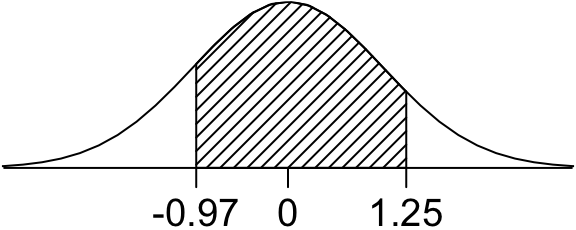
\includegraphics[width=0.45\linewidth]{ch05_24spr_ex_files/figure-beamer/unnamed-chunk-19-1} \end{center}

\scriptsize
\tabcolsep=3pt

\begin{tabular}[t]{l|r|r|>{}r|r|r|r|r|r|r|r}
\hline
  & 0.09 & 0.08 & 0.07 & 0.06 & 0.05 & 0.04 & 0.03 & 0.02 & 0.01 & 0.00\\
\hline
-1 & 0.1379 & 0.1401 & \cellcolor{lightgray}{0.1423} & 0.1446 & 0.1469 & 0.1492 & 0.1515 & 0.1539 & 0.1562 & 0.1587\\
\hline
\cellcolor{lightgray}{-0.9} & \cellcolor{lightgray}{0.1611} & \cellcolor{lightgray}{0.1635} & \cellcolor{lightgray}{0.1660} & \cellcolor{lightgray}{0.1685} & \cellcolor{lightgray}{0.1711} & \cellcolor{lightgray}{0.1736} & \cellcolor{lightgray}{0.1762} & \cellcolor{lightgray}{0.1788} & \cellcolor{lightgray}{0.1814} & \cellcolor{lightgray}{0.1841}\\
\hline
-0.8 & 0.1867 & 0.1894 & \cellcolor{lightgray}{0.1922} & 0.1949 & 0.1977 & 0.2005 & 0.2033 & 0.2061 & 0.2090 & 0.2119\\
\hline
\end{tabular}

\begin{tabular}[t]{l|r|r|r|r|r|>{}r|r|r|r|r}
\hline
  & 0.00 & 0.01 & 0.02 & 0.03 & 0.04 & 0.05 & 0.06 & 0.07 & 0.08 & 0.09\\
\hline
1.1 & 0.8643 & 0.8665 & 0.8686 & 0.8708 & 0.8729 & \cellcolor{lightgray}{0.8749} & 0.8770 & 0.8790 & 0.8810 & 0.8830\\
\hline
\cellcolor{lightgray}{1.2} & \cellcolor{lightgray}{0.8849} & \cellcolor{lightgray}{0.8869} & \cellcolor{lightgray}{0.8888} & \cellcolor{lightgray}{0.8907} & \cellcolor{lightgray}{0.8925} & \cellcolor{lightgray}{0.8944} & \cellcolor{lightgray}{0.8962} & \cellcolor{lightgray}{0.8980} & \cellcolor{lightgray}{0.8997} & \cellcolor{lightgray}{0.9015}\\
\hline
1.3 & 0.9032 & 0.9049 & 0.9066 & 0.9082 & 0.9099 & \cellcolor{lightgray}{0.9115} & 0.9131 & 0.9147 & 0.9162 & 0.9177\\
\hline
\end{tabular}

\normalsize

Ans \(= 0.8944-0.1660= 0.7284\).
\end{frame}

\begin{frame}{Example: 25th Percentile of the Standard Normal}
\protect\hypertarget{example-25th-percentile-of-the-standard-normal}{}
The 25th percentile of the standard normal is the \(z\) that

\vspace{-6pt}

\begin{center}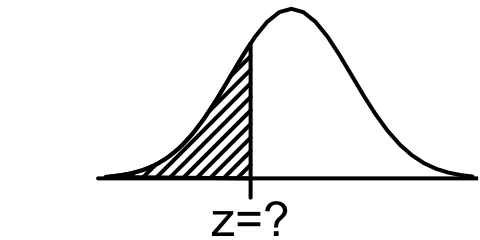
\includegraphics[width=0.3\linewidth]{ch05_24spr_ex_files/figure-beamer/unnamed-chunk-21-1} \end{center}
\vspace{-0.8in}

\[
\text{shaded area}\hspace{.25\textwidth}= 0.25.
\]

\vspace{8pt}

We need to search in the \red{body} of the normal table for the values
closest to 0.25, which are 0.2514 and 0.2483, and find the \(z\)
corresponding to those values, which are \(-0.67\) and \(-0.68\).

\begin{center}
%\renewcommand{\arraystretch}{0.85}
\tabcolsep=3pt\footnotesize
\only<1|handout:0>{
\begin{tabular}{c|cccccccccc}\hline
\alert{\small z}
      & {\footnotesize .00}   & {\footnotesize .01}   & {\footnotesize .02}   & {\footnotesize .03} & {\footnotesize .04}   & {\footnotesize .05} & {\footnotesize .06}   & {\footnotesize .07}   & {\footnotesize .08}   & {\footnotesize .09} \\\hline
$\vdots$&$\vdots$&$\vdots$&$\vdots$&$\vdots$&$\vdots$&$\vdots$&$\vdots$&$\vdots$&$\vdots$&$\vdots$\\
%$-0.8$& .2119 & .2090 & .2061 & .2033 & .2005 & .1977 & .1949 & .1922 & .1894 & .1867\\
$-0.7$& .2420 & .2389 & .2358 & .2327 & .2296 & .2266 & .2236 & .2206 & .2177 & .2148\\
$-0.6$& .2743 & .2709 & .2676 & .2643 & .2611 & .2578 & .2546 & .2514 & .2483 & .2451\\
$-0.5$& .3085 & .3050 & .3015 & .2981 & .2946 & .2912 & .2877 & .2843 & .2810 & .2776\\[-2pt]
%$-0.4$& .3446 & .3409 & .3372 & .3336 & .3300 & .3264 & .3228 & .3192 & .3156 & .3121\\
$\vdots$&$\vdots$&$\vdots$&$\vdots$&$\vdots$&$\vdots$&$\vdots$&$\vdots$&$\vdots$&$\vdots$&$\vdots$\\\hline
\end{tabular}
}\only<2->{
\begin{tabular}{c|ccccccc>{\columncolor[gray]{0.7}[1pt]}c>{\columncolor[gray]{0.7}[1pt]}cc}\hline
\alert{\small z}
      & {\footnotesize .00}   & {\footnotesize .01}   & {\footnotesize .02}   & {\footnotesize .03} & {\footnotesize .04}   & {\footnotesize .05} & {\footnotesize .06}   & {\footnotesize .07}   & {\footnotesize .08}   & {\footnotesize .09} \\\hline
$\vdots$&$\vdots$&$\vdots$&$\vdots$&$\vdots$&$\vdots$&$\vdots$&$\vdots$&$\vdots$&$\vdots$&$\vdots$\\
%$-0.8$& .2119 & .2090 & .2061 & .2033 & .2005 & .1977 & .1949 & .1922 & .1894 & .1867\\
$-0.7$& .2420 & .2389 & .2358 & .2327 & .2296 & .2266 & .2236 & .2206 & .2177 & .2148\\
\rowcolor[gray]{0.7}$-0.6$& .2743 & .2709 & .2676 & .2643 & .2611 & .2578 & .2546 & \alert{.2514} & \alert{.2483} & .2451\\
$-0.5$& .3085 & .3050 & .3015 & .2981 & .2946 & .2912 & .2877 & .2843 & .2810 & .2776\\[-2pt]
$\vdots$&$\vdots$&$\vdots$&$\vdots$&$\vdots$&$\vdots$&$\vdots$&$\vdots$&$\vdots$&$\vdots$&$\vdots$\\\hline
\end{tabular}
}
\end{center}
\end{frame}

\begin{frame}{Example: 95th Percentile of the Standard Normal}
\protect\hypertarget{example-95th-percentile-of-the-standard-normal}{}
The 95th percentile of the standard normal is the \(z\) such that\\
\vspace{-6pt}

\begin{center}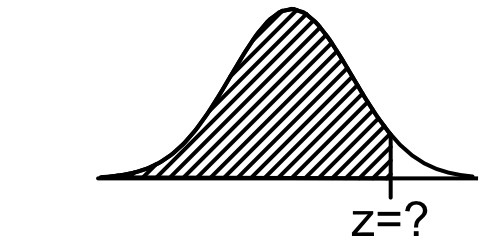
\includegraphics[width=0.3\linewidth]{ch05_24spr_ex_files/figure-beamer/unnamed-chunk-22-1} \end{center}
\vspace{-0.8in}

\[
\text{shaded area}\hspace{.25\textwidth}= 0.95.
\]

\bigskip
\begin{center}
\footnotesize
\tabcolsep=3pt
\begin{tabular}{c|cccc>{\columncolor[gray]{0.7}[1pt]}c>{\columncolor[gray]{0.7}[1pt]}ccccc}\hline
\alert{\normalsize z}
     & {\footnotesize .00}   & {\footnotesize .01}   & {\footnotesize .02}   & {\footnotesize .03} & {\footnotesize .04}   & {\footnotesize .05} & {\footnotesize .06}   & {\footnotesize .07}   & {\footnotesize .08}   & {\footnotesize .09} \\\hline
$1.5$& .9332 & .9345 & .9357 & .9370 & .9382 & .9394 & .9406 & .9418 & .9429 & .9441\\
\rowcolor[gray]{0.7}$1.6$& .9452 & .9463 & .9474 & .9484 & \alert{.9495} & \alert{.9505} & .9515 & .9525 & .9535 & .9545\\
$1.7$& .9554 & .9564 & .9573 & .9582 & .9591 & .9599 & .9608 & .9616 & .9625 & .9633\\\hline
\end{tabular}
\end{center}

The values closest to 0.95 in the body of the normal table are 0.9495
and 0.9505, corresponding to \(z\)-values 1.64 and 1.65.

The 95th percentile is thus between 1.64 and 1.65.
\end{frame}

\begin{frame}{In-Class Exercise 2}
\protect\hypertarget{in-class-exercise-2}{}
Find the 30th percentile of the standard normal curve.\pause

\scriptsize
\tabcolsep=3pt

\begin{tabular}[t]{l|r|r|r|r|r|r|>{}r|>{}r|r|r}
\hline
  & 0.09 & 0.08 & 0.07 & 0.06 & 0.05 & 0.04 & 0.03 & 0.02 & 0.01 & 0.00\\
\hline
-0.6 & 0.2451 & 0.2483 & 0.2514 & 0.2546 & 0.2578 & 0.2611 & \cellcolor{lightgray}{0.2643} & \cellcolor{lightgray}{0.2676} & 0.2709 & 0.2743\\
\hline
\cellcolor{lightgray}{-0.5} & \cellcolor{lightgray}{0.2776} & \cellcolor{lightgray}{0.2810} & \cellcolor{lightgray}{0.2843} & \cellcolor{lightgray}{0.2877} & \cellcolor{lightgray}{0.2912} & \cellcolor{lightgray}{0.2946} & \cellcolor{lightgray}{0.2981} & \cellcolor{lightgray}{0.3015} & \cellcolor{lightgray}{0.3050} & \cellcolor{lightgray}{0.3085}\\
\hline
-0.4 & 0.3121 & 0.3156 & 0.3192 & 0.3228 & 0.3264 & 0.3300 & \cellcolor{lightgray}{0.3336} & \cellcolor{lightgray}{0.3372} & 0.3409 & 0.3446\\
\hline
\end{tabular}

\normalsize

The 30th percentile is thus between \(-0.52\) and \(-0.53\).
\end{frame}

\begin{frame}{In-Class Exercise 3}
\protect\hypertarget{in-class-exercise-3}{}
Find the 82nd percentile of the standard normal curve.\pause

\scriptsize
\tabcolsep=3pt

\begin{tabular}[t]{l|r|>{}r|>{}r|r|r|r|r|r|r|r}
\hline
  & 0.00 & 0.01 & 0.02 & 0.03 & 0.04 & 0.05 & 0.06 & 0.07 & 0.08 & 0.09\\
\hline
0.8 & 0.7881 & \cellcolor{lightgray}{0.7910} & \cellcolor{lightgray}{0.7939} & 0.7967 & 0.7995 & 0.8023 & 0.8051 & 0.8078 & 0.8106 & 0.8133\\
\hline
\cellcolor{lightgray}{0.9} & \cellcolor{lightgray}{0.8159} & \cellcolor{lightgray}{0.8186} & \cellcolor{lightgray}{0.8212} & \cellcolor{lightgray}{0.8238} & \cellcolor{lightgray}{0.8264} & \cellcolor{lightgray}{0.8289} & \cellcolor{lightgray}{0.8315} & \cellcolor{lightgray}{0.8340} & \cellcolor{lightgray}{0.8365} & \cellcolor{lightgray}{0.8389}\\
\hline
1 & 0.8413 & \cellcolor{lightgray}{0.8438} & \cellcolor{lightgray}{0.8461} & 0.8485 & 0.8508 & 0.8531 & 0.8554 & 0.8577 & 0.8599 & 0.8621\\
\hline
\end{tabular}

\normalsize

The 82nd percentile is thus between 0.91 and 0.92.
\end{frame}

\begin{frame}{The Normal Approximation, An Example}
\protect\hypertarget{the-normal-approximation-an-example}{}
\newcommand\inch{{\tt "}}
\newcommand\foot{{\tt '}}

Consider the heights of women in HANES:

\begin{center}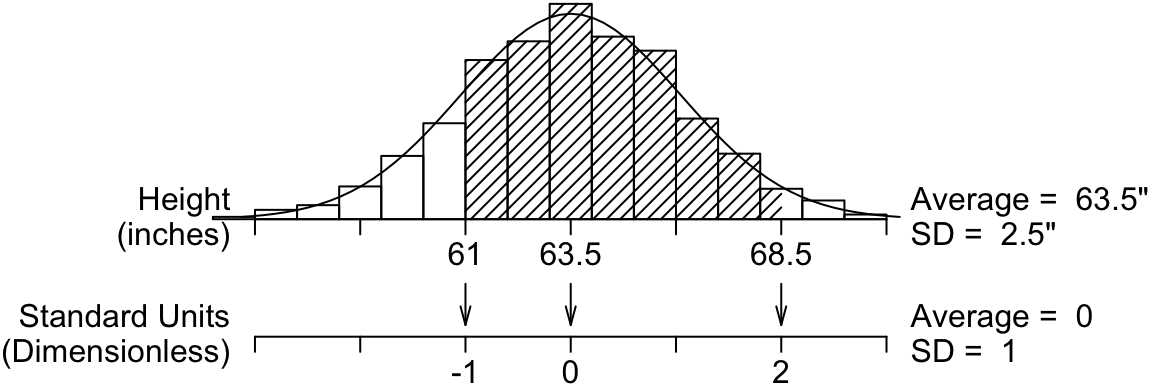
\includegraphics[width=1\linewidth]{ch05_24spr_ex_files/figure-beamer/NormApp-1} \end{center}

What percentage of women are between 61 and 68.5 inches tall?
\end{frame}

\begin{frame}{Standard Units}
\protect\hypertarget{standard-units}{}
\textbf{Standard units} say how many SDs a value is above (\(+\) sign)
or below (\(-\) sign) average.

\bigskip

\underline{Example}: the women in the HANES study had heights averaging
to 63.5{\tt "}, with an SD of 2.5{\tt "}.

\begin{enumerate}
\tightlist
\item
  What is 61{\tt "} in standard units?

  \begin{itemize}
  \tightlist
  \item
    61{\tt "} is \Hide{2-}{2.5} inches \Hide{2-}{below} average.
  \item
    That's \Hide{3-}{1} SD \Hide{3-}{below} average.
  \item
    So 61{\tt "} is \Hide{4-}{$-1$} in standard units.
  \end{itemize}
\item
  What is 68.5{\tt "} in standard units?

  \begin{itemize}
  \tightlist
  \item
    68.5{\tt "} is \Hide{5-}{5} inches \Hide{5-}{above} average.
  \item
    That's \Hide{6-}{2} SD \Hide{6-}{above} average.
  \item
    So 68.5{\tt "} is \Hide{7-}{$+2$} in standard units.
  \end{itemize}
\end{enumerate}
\end{frame}

\begin{frame}{Standard Units (Cont'd)}
\protect\hypertarget{standard-units-contd}{}
\underline{Example}: the women in the HANES study had heights averaging
to 63.5{\tt "}, with an SD of 2.5{\tt "}.

\begin{enumerate}
\setcounter{enumi}{2}
\tightlist
\item
  What height is \(-2.4\) in standard units?

  \begin{itemize}
  \tightlist
  \item
    The height is \Hide{2-}{2.4} SDs \Hide{3-}{below} average.
  \item
    That's \Hide{4-}{$2.4\times 2.5=6$} inches \Hide{4-}{below} average.
  \item
    The height is \Hide{5-}{$63.5-6=57.5${\tt "}}.
  \end{itemize}
\end{enumerate}

\bigskip

\begin{center}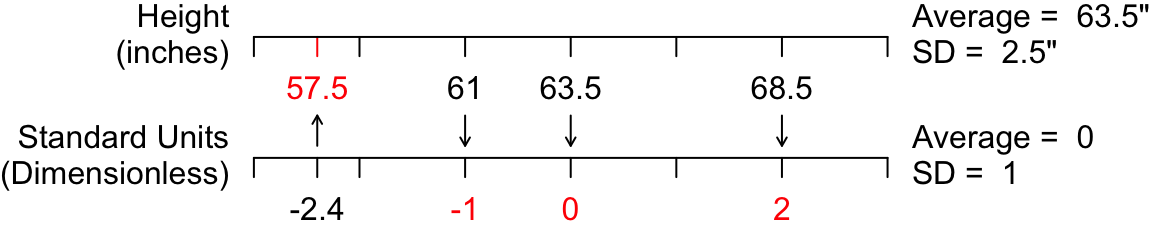
\includegraphics[width=1\linewidth]{ch05_24spr_ex_files/figure-beamer/unnamed-chunk-25-1} \end{center}
\end{frame}

\begin{frame}{Original Scale \(\Leftrightarrow\) Standard-Unit Scale}
\protect\hypertarget{original-scale-leftrightarrow-standard-unit-scale}{}
How to convert a value to standard units?

\begin{center}
\fboxrule=1pt
\fboxsep=8pt
\fbox{standard units $\displaystyle{= \frac{\text{value} - \text{average}}{\text{SD}}.}$}
\end{center}

E.g., to express 68.5{\tt "} in standard units, you compute \[
\frac{68.5{\tt "}- 63.5{\tt "}}{2.5{\tt "}}=\frac{5.0{\tt "}}{2.5{\tt "}} =2
\]

\hrule\medskip

How to convert to the original scale back from standard units?

\begin{center}
\fboxrule=1pt
\fboxsep=8pt
\fbox{value $\displaystyle{= \text{average} + (\text{standard units}\times\text{SD}).}$}
\end{center}

E.g., to find the height corresponding to \(-2.4\) in standard units,
you compute
\[ 63.5{\tt "}+ (-2.4 \times 2.5{\tt "}) = 63.5{\tt "}- 6{\tt "}= 57.5{\tt "}\]
\end{frame}

\begin{frame}{Back to the Normal Approximation Example}
\protect\hypertarget{back-to-the-normal-approximation-example}{}
\begin{center}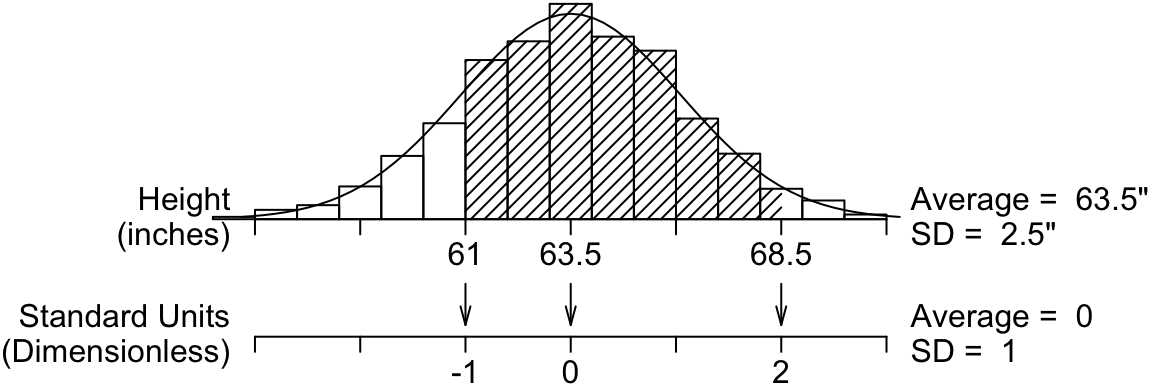
\includegraphics[width=1\linewidth]{ch05_24spr_ex_files/figure-beamer/unnamed-chunk-26-1} \end{center}

The percentage of women between 61{\tt "} and 68.5{\tt "} tall is

\begin{itemize}
\tightlist
\item
  \underline{exactly} equal to the area under the \underline{histogram}
  from 61{\tt "} to 68.5{\tt "}, and
\item
  \underline{approximately} equal to the area under the
  \underline{normal curve} between \(-1\) and 2. See next page.
\end{itemize}
\end{frame}

\begin{frame}{}
\protect\hypertarget{section-6}{}
\vspace{6pt}
\begin{minipage}{0.75\textwidth}
It remains to find the \textbf{area} under the 
standard normal curve \textbf{between} $-1$ and 2.
\end{minipage}
\vspace{-0.6in}

\begin{flushright}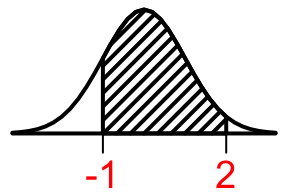
\includegraphics[width=0.25\linewidth]{ch05_24spr_ex_files/figure-beamer/unnamed-chunk-27-1} \end{flushright}
\vspace{-6pt}
\footnotesize\tabcolsep=4pt
\begin{tabular}{@{}c|>{\columncolor[gray]{0.7}[1pt]}cccccccccc@{}}\hline
\alert{\small z}
      & {\footnotesize .00}   & {\footnotesize .01}   & {\footnotesize .02}   & {\footnotesize .03} & {\footnotesize .04}   & {\footnotesize .05} & {\footnotesize .06}   & {\footnotesize .07}   & {\footnotesize .08}   & {\footnotesize .09} \\\hline
$-1.1$& .1357 & .1335 & .1314 & .1292 & .1271 & .1251 & .1230 & .1210 & .1190 & .1170\\
\rowcolor[gray]{0.7}$-1.0$& \alert{.1587} & .1562 & .1539 & .1515 & .1492 & .1469 & .1446 & .1423 & .1401 & .1379\\
$-0.9$& .1841 & .1814 & .1788 & .1762 & .1736 & .1711 & .1685 & .1660 & .1635 & .1611\\
$\vdots$&$\vdots$&$\vdots$&$\vdots$&$\vdots$&$\vdots$&$\vdots$&$\vdots$&$\vdots$&$\vdots$&$\vdots$\\
$1.9$& .9713 & .9719 & .9726 & .9732 & .9738 & .9744 & .9750 & .9756 & .9761 & .9767\\
\rowcolor[gray]{0.7}$2.0$& \alert{.9772} & .9778 & .9783 & .9788 & .9793 & .9798 & .9803 & .9808 & .9812 & .9817\\
$2.1$& .9821 & .9826 & .9830 & .9834 & .9838 & .9842 & .9846 & .9850 & .9854 & .9857\\\hline
\end{tabular}\normalsize\par

\begin{center}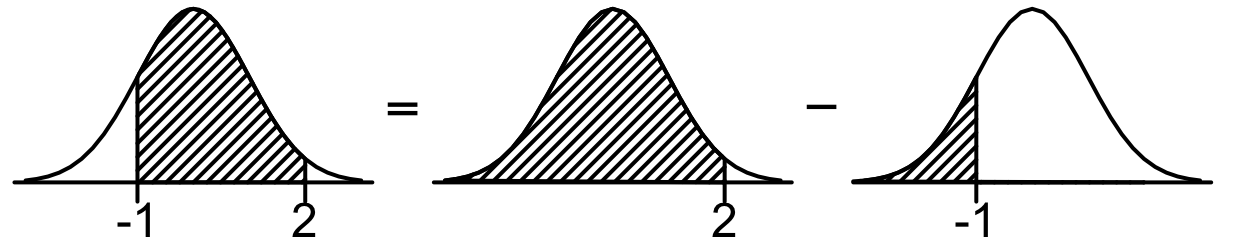
\includegraphics[width=0.8\linewidth]{ch05_24spr_ex_files/figure-beamer/unnamed-chunk-28-1} \end{center}

\vspace{-0.4in}

\[
\qquad\qquad=\alert{0.9772}-\alert{0.1587}=0.8185
\] \pause Answer: 81.85\%
\end{frame}

\begin{frame}{The Normal Approximation (Cont'd)}
\protect\hypertarget{the-normal-approximation-contd}{}
\begin{itemize}
\item
  If a list of numbers follows the normal curve, the percentage of
  entries falling in a given interval can be estimated by first
  converting the interval to standard units and then finding the
  corresponding area under the standard normal curve. This procedure is
  called the \textbf{normal approximation}.
\item
  If a histogram follows the normal curve,

  \begin{itemize}
  \tightlist
  \item
    about 68\% of the area lies within one SD of the average, and
  \item
    about 95\% within two SDs of the average.
  \end{itemize}
\item
  \textbf{Warning}: The normal approximation is only valid if the
  \underline{histogram is approximately normal}. Use your judgement.
\end{itemize}
\end{frame}

\begin{frame}{Using the Normal Approximation}
\protect\hypertarget{using-the-normal-approximation}{}
A group of men have heights that follow a normal curve with average
69{\tt "} and SD 3. About what percentage of them are below
66{\tt "} tall? \vspace{-0.2in}

\begin{flushleft}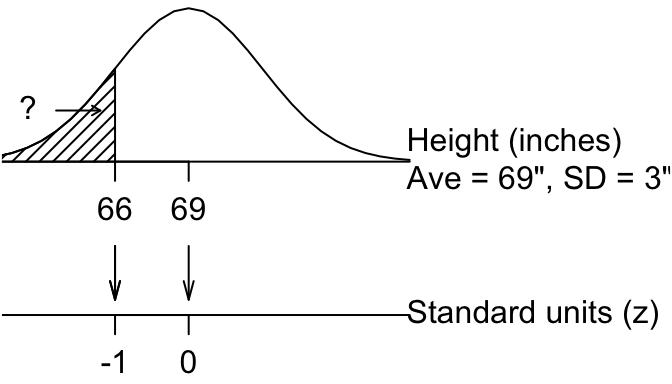
\includegraphics[width=0.55\linewidth]{ch05_24spr_ex_files/figure-beamer/unnamed-chunk-29-1} \end{flushleft}
\vspace{-1in}
\begin{flushright}
\scriptsize\tabcolsep=2pt
\begin{tabular}{@{}cccc>{\columncolor[gray]{0.7}[0pt]}c | c@{}}\hline
{\footnotesize 0.04} &  {\footnotesize 0.03} &  {\footnotesize 0.02} & {\footnotesize 0.01} &  {\footnotesize 0.00} & {\footnotesize$Z$}  \\  \hline 
.1271 & .1292 & .1314 & .1335 & .1357 & $-1.1$ \\
\rowcolor[gray]{0.7} .1492 & .1515 & .1539 & .1562 & \alert{.1587} & $-1.0$ \\
.1736 & .1762 & .1788 & .1814 & .1841 & $-0.9$ \\\hline
\end{tabular}
\end{flushright}

\begin{enumerate}
\tightlist
\item
  Sketch a normal curve, and shade area of interest
\item
  Convert 66{\tt "} to standard unit: \(z=\dfrac{66-69}{3}=-1\)
\item
  From Normal Table, the area to the left of \(-1\) is \alert{0.1587}.
\end{enumerate}

Answer: 15.87\% or about 16\%.\pause

Method: original units \(\rightarrow\) standard units \(\rightarrow\)
normal curve.
\end{frame}

\begin{frame}{}
\protect\hypertarget{section-7}{}
Same population (heights averaging to 69{\tt "} with an SD of 3{\tt "}).

How tall a man must be to be taller than 95\% of the population?

\begin{center}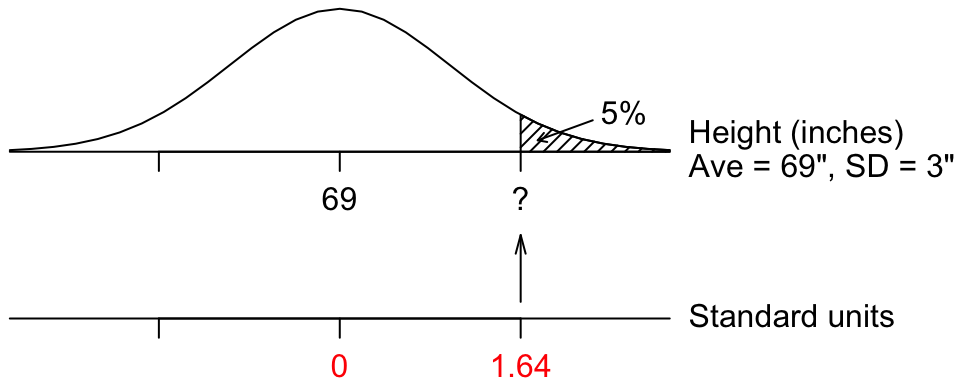
\includegraphics[width=0.8\linewidth]{ch05_24spr_ex_files/figure-beamer/unnamed-chunk-30-1} \end{center}

Thus \begin{align*}
\text{? = height} &= \text{\Hide{2-}{1.64} SDs above average}\cr
&= 1.64\times 3{\tt "}+ 69{\tt "}\cr
& = 5{\tt "}+ 69{\tt "}= 74{\tt "}= 6{\tt '}2{\tt "}
\end{align*} The method:\newline standard normal curve \(\rightarrow\)
standard units \(\rightarrow\) original units.
\end{frame}

\begin{frame}{}
\protect\hypertarget{section-8}{}
The general procedure for working these kinds of problems:

\begin{center}
\fboxrule=1pt
\fboxsep=8pt
\fbox{Draw the picture!}
\end{center}

\begin{itemize}
\tightlist
\item
  Sketch the normal curve
\item
  Put in the axis for the original units
\item
  Put in the axis for the standard units
\item
  Shade the area of interest
\item
  Proceed
\end{itemize}

\begin{center}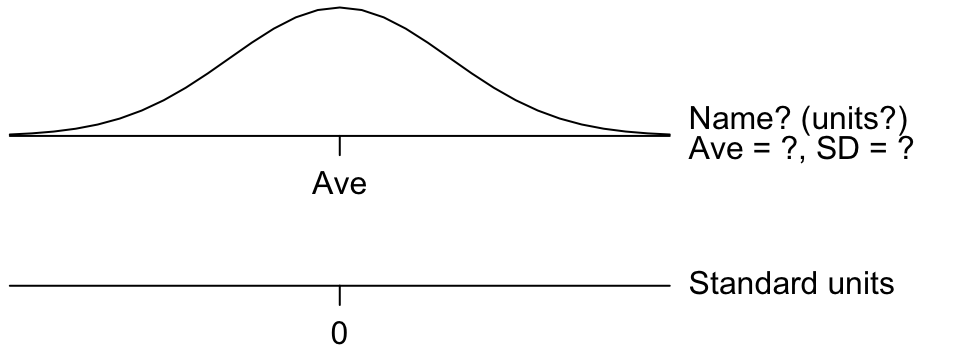
\includegraphics[width=0.9\linewidth]{ch05_24spr_ex_files/figure-beamer/unnamed-chunk-31-1} \end{center}

Follow this procedure on the HW, quizzes, and exams!
\end{frame}

\begin{frame}{General Procedure for Finding Normal Areas}
\protect\hypertarget{general-procedure-for-finding-normal-areas}{}
\begin{enumerate}
\tightlist
\item
  Sketch the normal curve
\item
  Put in the axis for the original units
\item
  Put in the axis for the standard units
\item
  Shade the area of interest
\item
  Convert end point (values) to standard units (z)
\item
  Find lower-tail area(s) for standard units from the normal table
\item
  Calculate the area of interest
\end{enumerate}

\begin{center}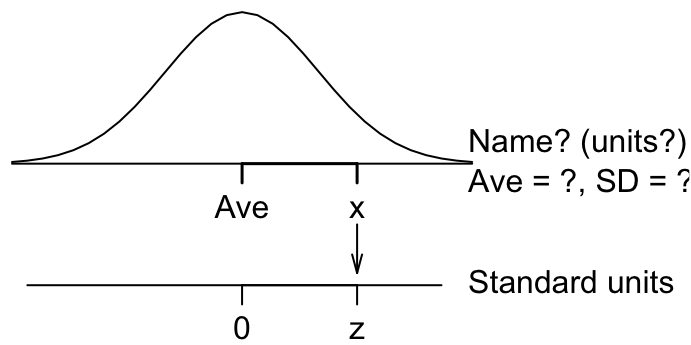
\includegraphics[width=0.7\linewidth]{ch05_24spr_ex_files/figure-beamer/unnamed-chunk-32-1} \end{center}
\end{frame}

\begin{frame}{General Procedure for Finding Normal Percentiles}
\protect\hypertarget{general-procedure-for-finding-normal-percentiles}{}
\begin{enumerate}
\tightlist
\item
  Sketch the normal curve
\item
  Put in the axis for the original variable \(X\)
\item
  Put in the axis for the standard units
\item
  Shade the area of interest
\item
  Find the standard unit \(z\) for the lower-tail area from the normal
  table
\item
  Find original value \(X\) (= percentile) from standard unit \(z\)
\end{enumerate}

\begin{center}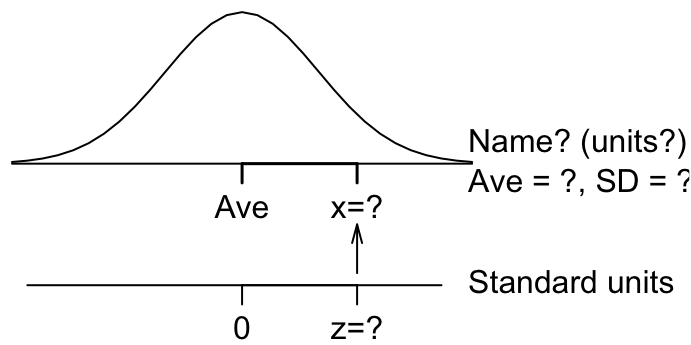
\includegraphics[width=0.7\linewidth]{ch05_24spr_ex_files/figure-beamer/unnamed-chunk-33-1} \end{center}
\end{frame}

\end{document}
